\RequirePackage[hyphens]{url}

\documentclass[sigconf]{acmart}

\usepackage{graphicx}
\usepackage{hyperref}
\usepackage{todonotes}

\usepackage{endfloat}
\renewcommand{\efloatseparator}{\mbox{}} % no new page between figures

\usepackage{booktabs} % For formal tables

\settopmatter{printacmref=false} % Removes citation information below abstract
\renewcommand\footnotetextcopyrightpermission[1]{} % removes footnote with conference information in first column
\pagestyle{plain} % removes running headers

\newcommand{\TODO}[1]{\todo[inline]{#1}}

\begin{document}
\title{Big Data Analytics in Indian Premier League}


\author{Swargam, Prashanth}

\affiliation{%
  \institution{Indiana University Bloomington}
  \streetaddress{107 S Indiana Ave}
  \city{Bloomington} 
  \state{Indiana} 
  \postcode{47408}
}
\email{pswargam@iu.edu}


% The default list of authors is too long for headers}
\renewcommand{\shortauthors}{G. v. Laszewski}


\begin{abstract}

Cricket is one of the most admired sports across the globe. Indian Premier League is one of the professional cricket leagues conducted by Board of Cricket Control India in the months of April and May. This league is famous for its diversity of players and breath-taking cricket match endings. The factors of winning change for each moment as the game progresses. As there are many players and franchises involved in the game, these factors for winning changes for each team. Data related to each player is required to analyse his performance and predict his future scope in team. Data related to factors of winning is crucial and can be analysed for predicting the results of the game. This analysis would help the team management, league administration to wisely chose the players and modify rules according to the impact of each decision. Data related some of the important factors which plays major role in deciding the match winner are analysed. Their impact is predicted and compared with the actual results. Impact of these factors are studied for each individual team and individual season of this cricket tournament. Impact of each factor is plotted and its impact in next season is predicted.

\end{abstract}

\keywords{Big Data, Cricket,Indian Premier League, i523}


\maketitle



\section{Introduction}

Fast paced games are gaining more importance in near future. This because there are many factors which contribute to the result of the game. These factors are minor but could change the results of the game dramatically. Indian Premier League is one such type of cricket league where there are a lot factors which have their influence on the results of the game. These factors are though minor or major, will have bigger part in deciding the results of the game. These factors from the previous games can be utilised wisely to predict their influence in the upcoming matches.  These factors can be quantitatively represented in the form numbers, graphs or Booleans. This quantitative representation of data related the factors can be analysed using various analytic techniques to predict their impact on the game.


	However, Analytics is a good way to go about this prediction, but there are several problems which should be addressed. Considering the role of batsman, it will be having parameters like balls faced, dot balls, number of boundaries, strike rate etc. Considering the role of bowler, there are various parameters like matches played, overs bowled, economy rate. There are many similar kinds of roles in the game and above-mentioned parameters are specific to one player playing only one role in the team. According to, around 500 players play for each season of cricket. These 500 players will be filtered on various factor from the pool of nearly 5,31,253 cricket players across the globe. These players can play any of the role or play multiple to roles to contribute to the result of the match. These players and cricket matches produces large amount of data which when analysed to produce structured data and analytics. Hence, there is good scope of analytics ad big data in this sport.
	
	
	The data produced by the matches happening in Indian Premier League can be used to fit in mathematical models. These mathematical models are then used to study the nature and trends of the factors which influence the results of the game. Extending this model to the known values of the input factors can produce the predicted values of the impacts of these factors. Models like Linear regression, polynomial regression, radial-basis approach can be applied to do these kinds of predictive analysis. 



\section{Problem Statement}

There are various factors influencing the results of the game. As part of this analytics, data related to four of the most influencing factors is gathered and modelled for analysis. This data was available in raw formats which requires some amount of modelling for predictive analysis. The modelled data is used for building a mathematical model which would fit closely to the trend of these factors in matches played in all the past seasons. A part of data is assumed to be unknown. This unknown part of data is predicted by using the fitted mathematical models. Results obtained by these predictions are compared with the actual results from the data source. Impact of these factors are calculated to the ratio of one. These data is analysed for each independent team and each independent season.

 
The report is in regard to the predictive analysis conducted on only five of the most influencing factors in the game. There are other factors in the game which might influence the result of the game. This predictive analysis will only be considered reliable only if the predicted values of the results will have high accuracy with respect to the actual results of the available data. The data is divided into two parts. All the available data is sorted with respect to date. The latest match comes later in the dataset and the earliest first. The first part of data is used to train the mathematical model. The parameters in the later part of the dataset are used to predict the result of the match. These predicted results are then compared with the actual results in the datasets to determine the accuracy of the predictive model which is used to build the analytics. This analysis produce valuable insights on the influence of these factors and the mathematical model.


\section{Scope}

The scope of the analysis is:


1)The analytics uses the data for only five factors. These five factors are  namely toss, Batting position, Range of score, portion of runs in boundaries.


2)The data is collected for all the seasons completed for this tournament. However, this data is sorted with respect to date and partitioned into training and testing data sets for calculating the accuracy of the model.


3) The values of these factors are represented in usable data formats like range, Boolean, integers for analysis.


\section{Factors in Consideration}

\subsection{Batting Sequence}
Order of batting is considered as one of the factors in consideration. Batting order is one crucial parameter which depends on various other factors of the game. Some of these parameters are the status of the pitch for the game, climate conditions of the game, previous statistics of the game and the history of the team in similar situations. The toss winner will have the privilege to decide the order of the batting. As this factor is conglomeration of various other factors stated above, batting order is considered for the analytics. This data can be represented in the form of Boolean. Where true Boolean indicates that the team referring to the statistics have batted first in the game. False indicates that the team referring to the statistics have batted second in the game.  This Boolean value depends on the values in for toss winner and toss decision.
\subsection{Total Score}
Score indicates the total number of runs scored by the team in any match. Score of the team depends on various other parameters of the game like team statistics and composition, impact of the opponents, and situation of the match. This parameter can be calculated from other values of extra runs, scored runs. This categorized into four categories. This first category of the innings scored not more than 100 runs. The second category of the innings scored more than 100 and less than 150 runs. The third category of the innings scored more than 150 and less than 200 hundred runs. All the other innings which scored more than 200 are categorised into fourth category. This categorization is done in accordance to the range of scores. The least scored innings were given least category value. The highest scored innings were given highest category value.
\subsection{Score Composition}
Composition of scored runs. The runs are majorly scored in the form of boundaries, players individual running,  and the extra runs given by then bowling team. As IPL is a T20 game which is played for short duration of time, scoring runs quickly at right time is crucial factor. Boundaries contribute to runs scored in the form of fours and sixes in the game. This is the easiest way to quickly score the runs. Team scoring high majority of runs in the form of boundaries have higher chance of imposing a higher target to the opponents or chasing down the target imposed by the opponents. Hence, this parameter is considered for analysis. This value for this parameter is a Boolean. This value is set to true, if most of the runs scored by any team in any innings are from boundaries and vice versa.

\subsection{Toss}
The batting sequence is decided by the winner of the toss. Winner of the toss will have the initial upper hand in the game to decide the sequence of the game. The winner’s decision will vary on various other factors of the game like, duration of the match, pitch behaviour throughout the game, statistics of the game. This various factors play an important role in deciding the toss winner’s decision. The value for this parameter is Boolean. The true value of the parameter indicates the team has won the toss and the false value indicates the team has not won the toss.

\section{Data Manipulation}

\subsection{Team data}
There are thirteen teams participated in IPL which was held for nine seasons. Each team was having its team name and teamId. These details are taken from the data source team.csv. Python’s csv module is used to read the data from this csv file. As this data represents a key value pair, csv module’s dictreader method is used to read the row in these files. Using this method, a dictionary was created which consisted of the teamId’s as keys and team name as value objects. 

\subsection{Match data}
 
Details pertaining to a specific match are published to the Match.csv file. These details include host team name, guest team name, toss winner id, match winner id, decision of the toss, win type. This data was used and modified for calculating the impact of each factors stated in the factors description. Python’s pandas dataframes were used to read the data from these csv files. All the missing values in the dataframes are replaced with 0 to ease the complexities that arise with null values. 
For each value in the team dictionary, the teamId is matched with the opponent team id column and team name id column in the match.csv. Python’s operator module is used to obtain the or condition between these values. Dataframe is modified with the given conditions .This dataframe is converted to list. This way, list of matches played by a team is defined and stored into a list.


From the dataframe which contains the list of matches played by the team, column matchwinnerid is used to define if the match winner. A new dataframe is created with a condition if the matchwinnerid’s value in the column is equals to the id of the current team. If the above-mentioned condition is true, then this value is added to the dataframe, else the value is removed from the dataframe. This way, list of matches won by a team is determined.


A new dataframe is created to store the Booleans of the toss decision. From the teamdata dataframe, the column toss winner id is used to determine the toss winner for each match. If the id value in this column is same as the team id of the current team, Boolean true is appended to the toss list. Else, Boolean false is appended to the toss list. This list contains only Booleans. 

\subsection{Ball-by-ball data}
Ball by ball analyses will be required to calculate the scores for each ball. These details will include the number of runs scored in the ball, extra runs scored, bowler details, batsman details, over details. This data is extracted from the ballbyball.csv file. This file contains ball by ball analysis of all the matches. This data is sorted according to the match id and is extracted for further analysis. Pandas readcsv method is used to read the csv file. A new data dataframe called balldata is created.


Balldata csv is used to for calculating the runs scored by a team in a specific match. The balldata dataframe is filtered for useless columns and null values. All the null values are replaced with 0 to ease the complexities which comes with usage of null values. Balldata’s team batting id and match id are used to calculate the runs scored by a team in a specific match. This data frame is modified such that, the values in the match id column is equal to the current match id and the values in the team batting id is equal to the current team id. Python operator module is used to achieve the and condition in the above case. 
The modified ball data data frame is used to calculate the score. The sum method on the dataframe is used from the pandas library. This score is categorised into four categories. The first category included the score which are less than hundred. The second category included the scores which are between hundred and one hundred fifty. The third category included the scores which are between one hundred fifty and two hundred. The fourth category of scores contain scores which are above two hundred. 


A new list is created which stored the category of the scores. If the score falls in first category, then an integer 1 is appended to the list. If the score falls in the second category, integer 2 is appended to the list. If the score falls in the category falls in the third category, an integer 3 is appended. If the score falls in the category four, an integer 4 is appended to the list.
The other factor which was stated in the factors in consideration team’s score composition. It is highly probable that a team scores a high total or chase down the target imposed by the opposition team quickly is the majority of runs are scored in the form of boundaries. The ball data dataframe which is created in the previous case is utilised with other conditions to calculate the contribution of boundaries to the total score. This dataframe is filtered with the match id and team id condition to obtain the current match and current batting team. This is again filtered for all the scores that are having values either four or six. The minified frame is filtered for all values of four and summed. The same is repeated with the sum of six values. Adding together these two sums will give the total amount of runs scored in form of boundaries.

A new list is created for storing the Booleans related to the contribution of boundaries to the score. This list is appended with value true, if the contribution of boundaries is more than other forms of runs, false if, the contribution of boundaries is less than the contribution of other forms of runs.

The lists which are created for each factor are used to define factors’ impact on the game’s result. These lists contain the values in the form of integers and Booleans which are obtained by using the existing parameters. These lists are created for each value in the team.csv file. Thus, they are independent to each team. A new DataFrame is created with these lists as columns in the frame. For each team, these frames are stored into another csv file using the pandas write csv function with the file name same as the value in the team dictionary.

\section{Predictive Analysis}

The factors and their values are written in to a csv file which contains the factor names as the columns headings and their respective values in the rows. Each team has its independent statistics files mentioned in the above statement. These files will be used for conducting the predictive analysis. For each value in the team dictionary, these csv files which are specific to the team are read using the pandas csv reader function.  There are two types of columns in these statistics file. The first type is predictors and the other type is targets. Columns related to the factors which impact the results are considered as the predictor columns, Columns related to the result of the match are considered as the targets column. Columns battingfirst, boundaries majority, wontoss, scorerange are predictors. Wonmatch column is target in the given scenario. 

The data available in the statistics files is split into test and train sets. This is done by the function train test split in the sklearn library in the python. The data is split in the ratio of 3 is to 2. Sixty percent of the data is used as training set. Forty percent of the data is used as testing set. The predictors and target of the training set are used to build the mathematical model. The predictors of the testing set are used to predict the values of the targets. These predicted values are compared with the actual target values. This comparision is used to determine the accuracy of the prediction.

\subsection{Implementation}

Decision trees and Random forest are used in making the predictions. Decision trees are tree like structures which are built based on the values of the parameters. These trees are useful in defining the probability of the target value being attained. Trees are build with various stems which are drawn from conditional statements. Decision trees has three kinds of elements. The first element i.e., are the decision elements which refer to the block which checks for the condition or logic of the tree. Chance elements are the elements which occur depending on the condition or logic of the function. End elements are the results or outcome of the decision tree. These are basically leaf nodes of the tree. These nodes represent the result. 
Random Forests are conglomeration of decisions from various decision trees. In random forest approach, a dataset is divided into various subsets which will have some or all the input parameters as the decision makers and some or all the data which are the values for the parameters. Each subset is used to build a tree by using principles of decision tree. The predictions from these prediction trees are used in determining the final value. When a given set of input parameters are giving, they are predicted with all the decision trees developed by the forest. The outcome from all the decision trees are noted. The majority of these outputs is decided as result. This way, the errors which might arise in using only one decision tree can be eradicated. An error from one model of decision tree will be dominated by the results from all the other decision tree. 

Random forest classifier from the module sklearn is used to build the various decision trees and predict these values. Classifier type object is instantiated in the code/cite. This object is assigned with the RandomForestclassifier and an attribute called n estimator. The variable n estimator will define the number of decision trees to be build for the analysis. Fit function from the sklearn module is used to develop the model for the random forest algorithm. Fit function will take the training parameters and training targets as inputs. These are divided into fifty subsets in this scenario. Predict function is used to predict the value of the target given test predictor variable as inputs. 

\subsection{Accuracy}

Generation of only one decision tree as the model for the given training data would produce erroneous results. Using the random forests, fifty decision trees are built to predict the correct value of the target. This way, errors produced by one of the decision tree will be corrected by the predictions from the other trees.


In the graph \ref{f:treenumvsaccuracy}, the accuracy of using various number of decision trees are plotted against the number of decision trees. It can be observed that using less than five decision trees, the accuracy for the prediction for all the teams is around sixty percentage. As the number of decision trees increased, the accuracy of all the prediction is increased by at least ten percent. The hundred percent accuracy is because, those teams have played less number of games.

\section{Impact of factors}

This indicates the contribution of each factor for predicting the result of the game. These values will determine the probability of the value of result on any given values for the input variables. In the first step, the distinct values of the target value are noted. For all the distinct values of an input parameter from the set of values of one of the input parameter, the probability of different kind of results  are calculated. This calculation is repeated for the distinct values in the set of input parameter and summed at the end. This produces the importance of the feature. The above procedure is repeated for all the decision tree and all the value are averaged for getting the overall value of the importance feature for that feature. This procedure is repeated for all the input parameters. This will give the contribution of each parameter to the result values. 

\subsection{Batting First}

The first importance feature for all the teams are plotted in the graph \ref{f:BattingFirst} . It is clear from the graph that the importance feature batting first is highest for Rising Pune super giants. This indicates that this team have won most of their previous matches with while batting first in the game. While the Chennai Super kings and Kochi Tuskers are also high, but they are less than half. This indicates that batting first in the match will be a favourable condition for the above mentioned   teams. For all the other teams except Kings xi Punjab, Pune warriors and Sunrisers Hyderabad, the batting first importance factor is nearly around 0.1. This implies, out of all that matches which were present in the training set, these team batted first for only ten percent of the games. 

However, the total number matches should also be considered while validating this condition. Though the value for Kochi Tuskers is high, this might also be because they have played less number of matches and they have batted first in all the winning matches.

\subsection{Score Composition}

Score Composition composition is the combination of different ways of getting runs. For any high scoring and successful game, a team will have to score runs at faster rate. Hence, scoring runs in form of boundaries will help a team a lot in turning the match in their favour.  In the graph \ref{f:BoundariesMajority} , Contribution of this factor against each team is plotted. This graph summarises the contribution towards of the score composition factor towards the factor. This factor is very high for Kochi Tuskers team, because they have played considerably less number of games. 


A factor around 0.2 to 0.3 seems around the average value for all the teams. It is clearly seen from the graph that this factor is high for Rising Pune Supergiants. That means, out of all the matches this team have won in all the season, in most of the matches, this team have scored most of their runs in form of boundaries.  Then, Rajasthan royals and Delhi Daredevils are having next higher values. A lower value of this factor means, that out of all the matches which this specific team have won, they have scored most of them in form of another form. Sunrisers Hyderabad and Royal challengers are one such team.

 
This factor is calculated independent of the team composition. This factor can be normalised with respect to the team composition.

\subsection{Score Range}

Score is the total number of runs scored by a team in a specific innings of the match. This factor is categorised into four categories. Each category has a range of value for runs. Based, on this runs, the team is classified into categories. The first category of team will have scored less than hundred runs. The second category of team have scored less than one hundred fifty. The third category of team have scored less than two hundred runs. The remaining teams comes under the fourth category. 
  
  This categorisation is used as one factor in determining the results. From the graph, it can be seen that this value is very high for some of the teams and considerably less for other teams. A higher value of this factor means that out of all the matches the specific team has won, most of the matches they have scored the runs in the higher categories ,or out of all the matches they lost, they have scores in the lower categories of the score. 

 From the graph \ref{f:scorerange} ,It is clear that, teams Kolkatta Knight Risers and Sun Risers Hyderabad have a value around 0.6. This implies that the wonmatch of column for this teams was mostly decided by the score range category column. For the teams like Gujarat Lions and Rising Pune Super giants, this value is low. It can be inferred that the wonmatch column for this table is mostly decided by other columns in the team statistics table.
 
\subsection{Toss}

Toss is another important factor considered for this analysis. The winner of the toss has the power to decide the sequence of the match. This decision of the winning captain will effect the results of the match. Given this opportunity, any captian would take decision in favour their side. Hence, toss is one important factor in deciding the results of the match. 

A higher value of this factor implies, that out of all the matches the specific team has won, they have also won the toss in most of the matches. It also implies that the column wontoss have contributed a large amount to the target column. A lower value of this factor implies that out of all the matches a specific team has lost, most of the matches they have lost the toss. 

 From the graph \ref{f:Wontoss} it is clear that the this value is higher for teams Delhi Daredevils, Gujarat Lions and Royal challengers bangalore. This implies that out of the matches they have won, most of the matches they have won the toss. This implies toss is one of the important factor for this team to win a specific match. It is clear from the graph that this value is lower for teams like Kolkatta Knight risers. This implies that out of all the matches won by this team, they have won toss in less number of matches. This implies that toss is not one of the important factors for this team to win. 
 
For the other teams, this value is around 0.15 which is considered as average contribution. For these teams, toss decision have a fair impact on the decision of the match. The wontoss column in the team statistics  have contributed fair amount to the target column.

 
\section{Statistical Analysis}
This analysis will give the statistics of each factors and their importance in the previous matches for each team. This is done by gathering the data from the team statistics which is prepared as part of the first step in the predictive analysis. 

A dictionary of team names is prepared using the teams.csv file from the source. This file is read using the read csv method in the csv library. An empty is list is created for the factors batting order,score range, toss. As there is only one kind of value for all these factors, they are grouped and studied together. The score range is studied in a different program. 

These empty lists are used for storing the percentage contribution of each factor towards the results of analysis. In this case, the data is not divided into test and training sets. All the data in the data sets are taken into consideration. The values used in the analysis are the actuals value and no predictions are made in defining these values. 

For every element in the team dictionary, we iterate over the specific team statistics csv file created in the first step of this predictive analysis. From these csv files , we resd the columns battingsfirst, majorityscore, wontoss columns. For each columns in the csv file, we create a corresponding dataframe in the python program using the pandas dataframe.  This dataframes are constructed on based on two values. The wonmatch column value and the value of the factor being studied. We append the corresponding row to the dataframe only if both the conditions are satisfied. This kind of conditional statements can be achieved by python or operator. 

For every factor, now independent dataframes are defined after both the  conditions are satisfied. Total matches is the length of the csv file. From the above calculatethe percentage of the dataframe which we have captured with respect to the total length of the csv file. This percentage value determines the percentage contribution of the factor towards determining the winning chances of the team.

 These percentages are calculated for all the teams in the team dictionary. These values are stored in the respective factors list. This list is used for plotting the bar graphs using the pythons matplotlib.

\subsection{Analysis of individual team}
From the the lists of percentage contributions from the above anaylsis. Analysis of each factor and their contribution towards the individual team has been plotted in the graph. These plots are plotted against the team name and the percentage bars which show the percentage of each factor.Graph \ref{f:otherstats} has been plotted with above lists. 

For the team Kolkatta knight riders, out of all the matches they have won, in forty percentage of those matches, they have score majority of their score in form of boundaries. Out of all the matches they have won, they also won toss in thirty percentage of the matches and batted first in twenty percentage of the matches. This implies that the probability of winning a match for kolkatta Knight riders team is high if they score moajority of their score in form of boundaries. Then decision of toss and sequence of matches have considerable effect in the matches’ decision.

Team Royal Challengers bangalore have followed the same trend as the kolkatta team in the analysis. Out of all the matches they have won, they also scored majority of the runs in the form of boundaries. While ,out of these matches, they won only twenty percent of the tosses, they batted first in nearly twenty five percentage of the matches. Runs have been major contributing factor in this team also.

Chennai Super Kings have majority of their contribution from the toss factor and batting sequence factor together. That implies that, from the all the matches they have won, they either won the toss or batted first in the match. This implies that the team Chennai Super kings will have to win toss or bat first to win the match.


Teams punjab and Kochi Tuskers have followed trend similar to that of Kolkatta Knight risers and royal challengers bangalore. They scored majority of their score in the form of boundaries in nearly forty percent of the matches played by them. The other factors toss and batting sequence have contributed to nearly twenty percentage of their winnings. This implies that scoring majority of runs in form of boundaries will favour these teams. 


Mumbai Indians team have the second highest percentage contribution from the factors toss and batting sequence compared to other teams. This team also have third highes contribution from the score composition factor. That implies, this team have higher chance of winning given any factor. Though the value from the any one factor is against them, the other factor will over ride the effect of the previous factor.


Gujarat Lions have the highest contribution from the factor batting order. That implies, out of all the matches won by this team, they have scored majority of runs in the form of boundaries. The other two factors are considerably low. This implies that Gujarat team will have to score most of the runs in the form of boundaries to win the match.


It can be inferred from the graph that rising pune super giants have not won a match while batting first in the game. Out of all the matches won by them, they have either batted second in the game or score majority of runs in the form of boundaries.

Team Deccan chargers have almost same amount of contribution from all the three factors. This team is consistently performing in any values of the factors. They have good balance of the conditions in the previous games.

Team Pune warriors has the lowest values for the factors toss and sequence of the match. They are also have less contribution from the factor composition of score. This implies that this team is under performing in any given condition. 

\subsection{Analysis of Range of Scores}

The scores were divided into categories. This analysis will contribute the percentage contribution of each range of the score to the result of the matches played by the specific team. This analysis can be used as to determine the safe score range for every team. 


Team dictionary is taken from the team.csv file. The team statistics csv file which is created in the predictive analysis will be utilised for the value for range of scores. The values from the columns score range and wonmatch will be utilised. The data in this csv file is not partitioned into training and testing sets. This analysis is performed on complete data. No data is predicted in this analysis also. This is analysis on all the available data. 


For every value in the team dictionary, we locate the team statistics csv file which is generated as part of the predictive analysis. Four empty lists are generated to store the number of matches won by each team with score in the given score range. Total number matches can be calculated by using the length of team statistics csv file that is being studied upon. For every value in the team dictionary, we divide the csv file into four different data frames. Each data frame corresponds to each range of scores. This partition can be achieved by using pandas data frame.

This dataframe are extracted using the two conditions. They are the value of score range must be equal to the range we are fetching data for and the other condition is the wonmatch column must be true.  

After corresponding data frames are extracted from the team staistics csv, we calculate the percentage of each range data frame length against the total length of the team statistics csv. This percentage value will give us the percentage contribution of each range towards the result of the match.

\subsection{Graphical Analysis on scores}

From the graph \ref{f:scorestats}, it is clear that most of the wining scores fall in the second and third category. That implies for any team to win the match, it is most likely that the team must score atleast hundred runs in the match and come under second category or score atleast one hundred fifty runs and come under third category. 


Teams Gujarat lions and pune warriors have never won match scoring less than hundred runs or more than two hundred runs. This implies that the range from hundred to two hundred is the safe score range for these teams. Gujarat have won most number of matches scoring in the third category that is atleast scoring one hundred fifty runs and atmost two hundred runs. This is more safe zone for them. While, for pune warriors team they have almost similar winning percentage in both the categories. 
Teams rising pune supergiants and kochi have never won a game scoring more than two hundred runs. This might be bacuse, they have not scored more than two hundred runs in any given match or they have not won in the matches  in which they scored more than two hundred runs. That implies that they are having a safe scoring in the range of one hundred fifty and two hundred.


Sunrisers Hyderabad team has more contribution from the the second and third categories of scoring in the game compared to the other two teams. This indicates that they are consistent in this category of scoring than other teams. They do not have major difference in contribution from these categories. This indicates that they are consistently scoring around one hundred fifty mark score which makes the assumption that this team have good batting side. From the statistics on this team it is clear that they have also won matches scoring less than hundred. It is clear that they are also having a good bowling side as well. 

Team Royal Challengers bangalore has highest contribution from the fourth category of scoring when compared to other teams. That implies, the team royal challengers banglore have highest probability of winning the matches , if they are scoring more than two hundred runs in the match. Then their next contribution comes from the score range of third category. That implies this team has a good batting side. Because they are having high scoring percentages from the third and fourth categories. 

Following the royal challenger banglore team is Chennai super kings team. This team have contributions from all the four categories of the scoring range. This implies this team is fairly consistent in both the categories of the game. 

Team Mumbai Indians have the highest contribution from the third category of the scoring range after Gujarat lions. They are also having contributions from all the categories of range of scores. This will clearly show that Mumbai Indians team has an inconsistent batting team. If these totals are from the second innings, it can also be assumed that whenever their batsman failed to score many runs, bowler won the match. 

Kolkatta team has the highest contribution from the first category of scoring after Kochi team and Pune super giants. This implies that the above three teams have a good batting side. Scoring less than hundred and winning match is sight of team having a good bowling side. Upon having good contributions from category one, kolkatta knight riders also has good contributions from the other three categories as well. This implies, that this team not only has good bowling side,it also ahs a good batting side as well.
 
 
\section{Conclusion}

Predictive Data analytics have provided promising solutions to various problems in wide variety of fields. As part of this study, predictive and statistical data analytics on data related to a cricket League, Indian Premier league is conducted.  As part of predictive analytics, the available data is split into training and testing data sets. The values from the model are used to predict the target value. These values are compared to the original values for accuracy. Method of improving the accuracy of model is studied. This study would be useful to determine the impact of a factor on the result of the game. This analysis would help in predicting the results of the matches acuurately with the model developed from the training data.

Statistical analysis on the same data is conducted to get the details related to the impact of a factor quantitatively on a specific team. This analysis pertains to the available data and no predictions are done. This kind of analysis would be useful in determining the strengths of individual team. This kind of analysis can be conducted to the nature and strengths of each team.

\begin{acks}

  The author would like to thank Dr. Gregor von Laszewski for his
  support and suggestions to write this report.
  
  The author would like to thank assistant instructors for their support in completing this project.
  
  The author would like to acknowledge that the base data for the analysis is provided  by \cite{data} .
  

\end{acks}

\bibliographystyle{ACM-Reference-Format}
\bibliography{report} 

\appendix

\begin{figure}[!ht]
  \centering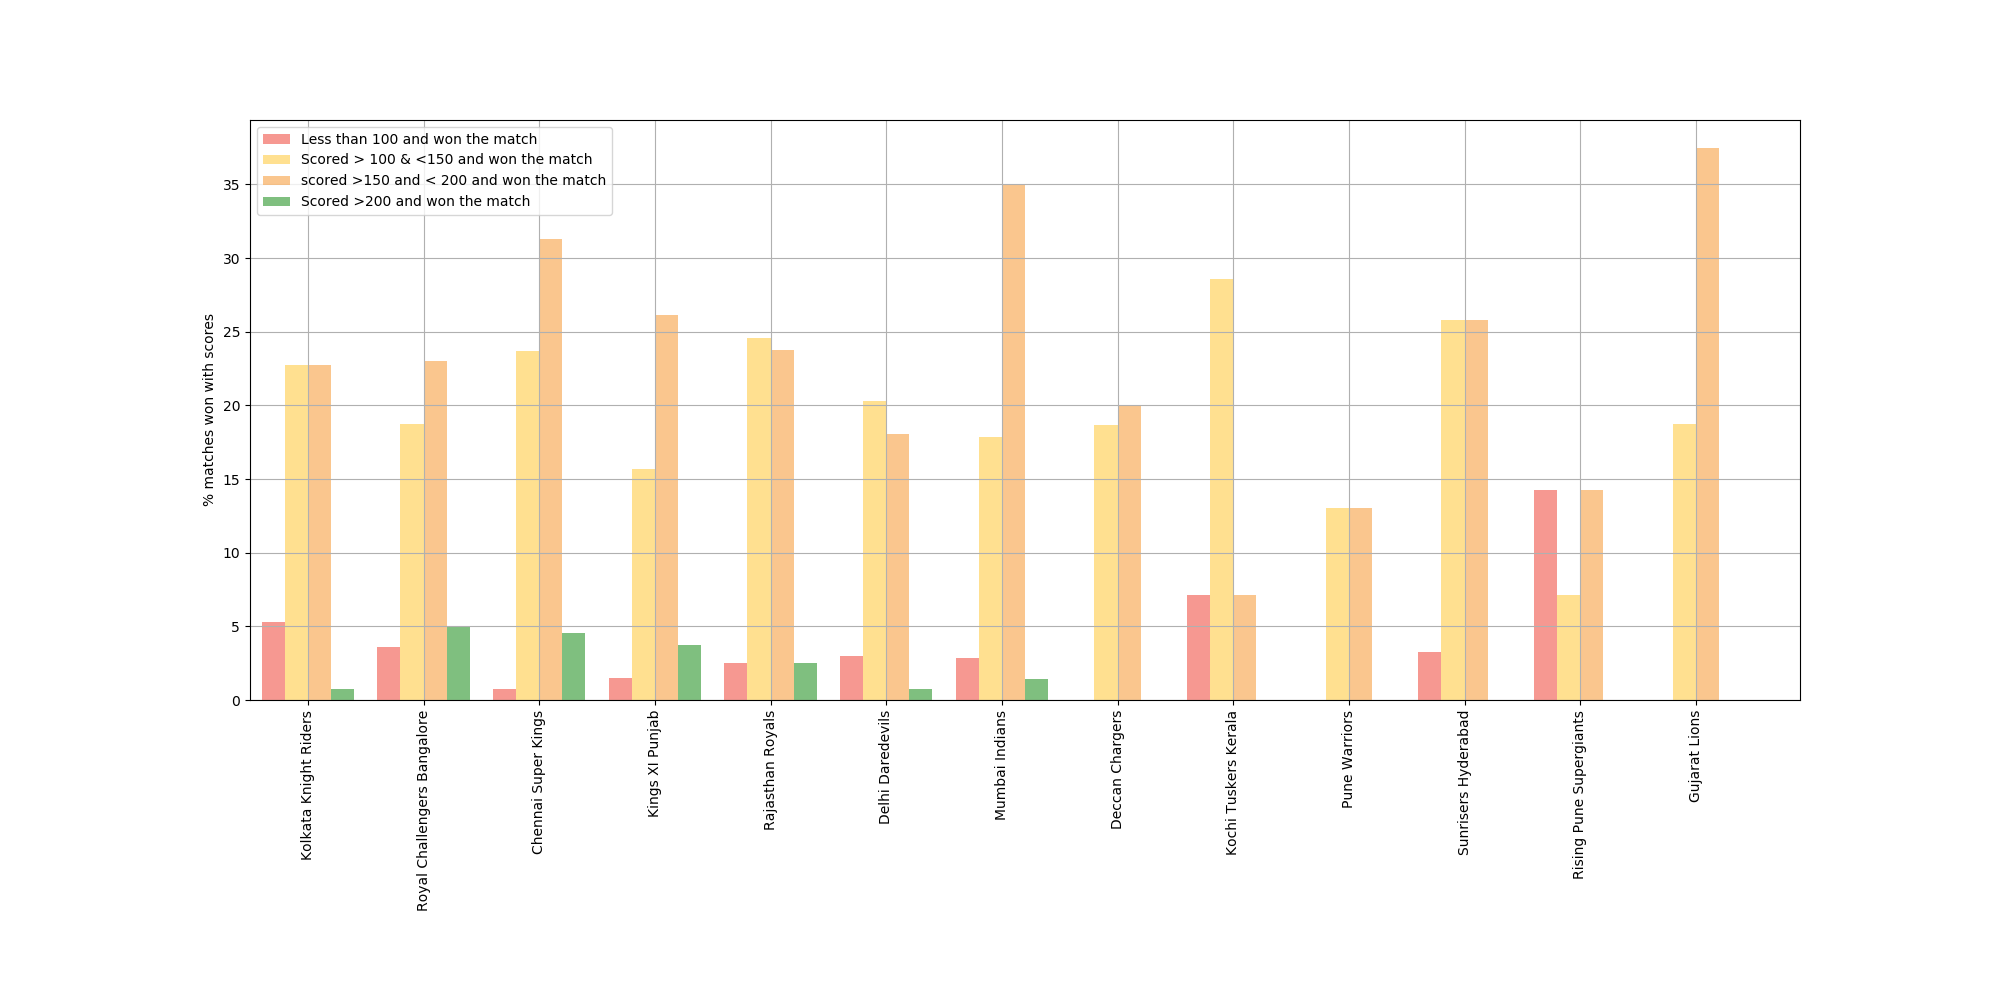
\includegraphics[width=\columnwidth]{images/scorestatictics.png}
  \caption{Score Staistics}\label{f:scorestats}
  
   \centering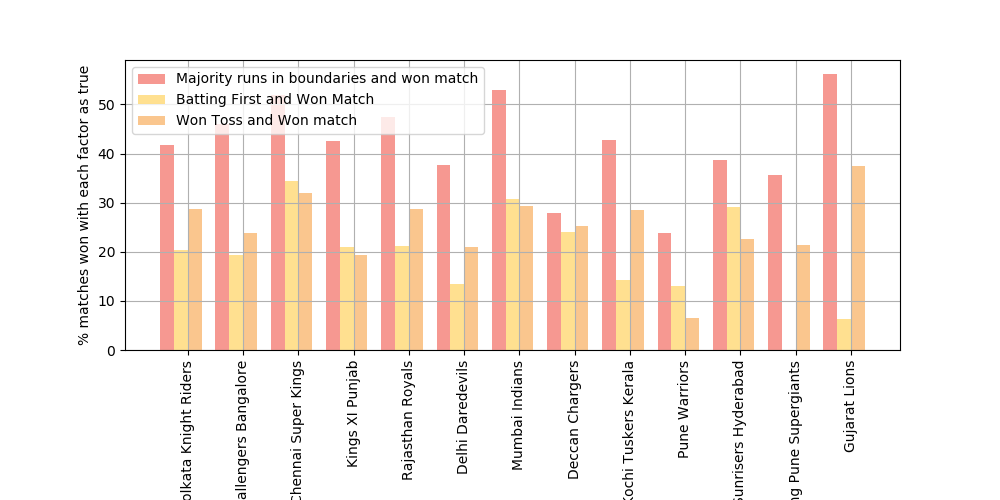
\includegraphics[width=\columnwidth]{images/otherstatistics.png}
  \caption{Other Factors Staistics}\label{f:otherstats}
  
  \centering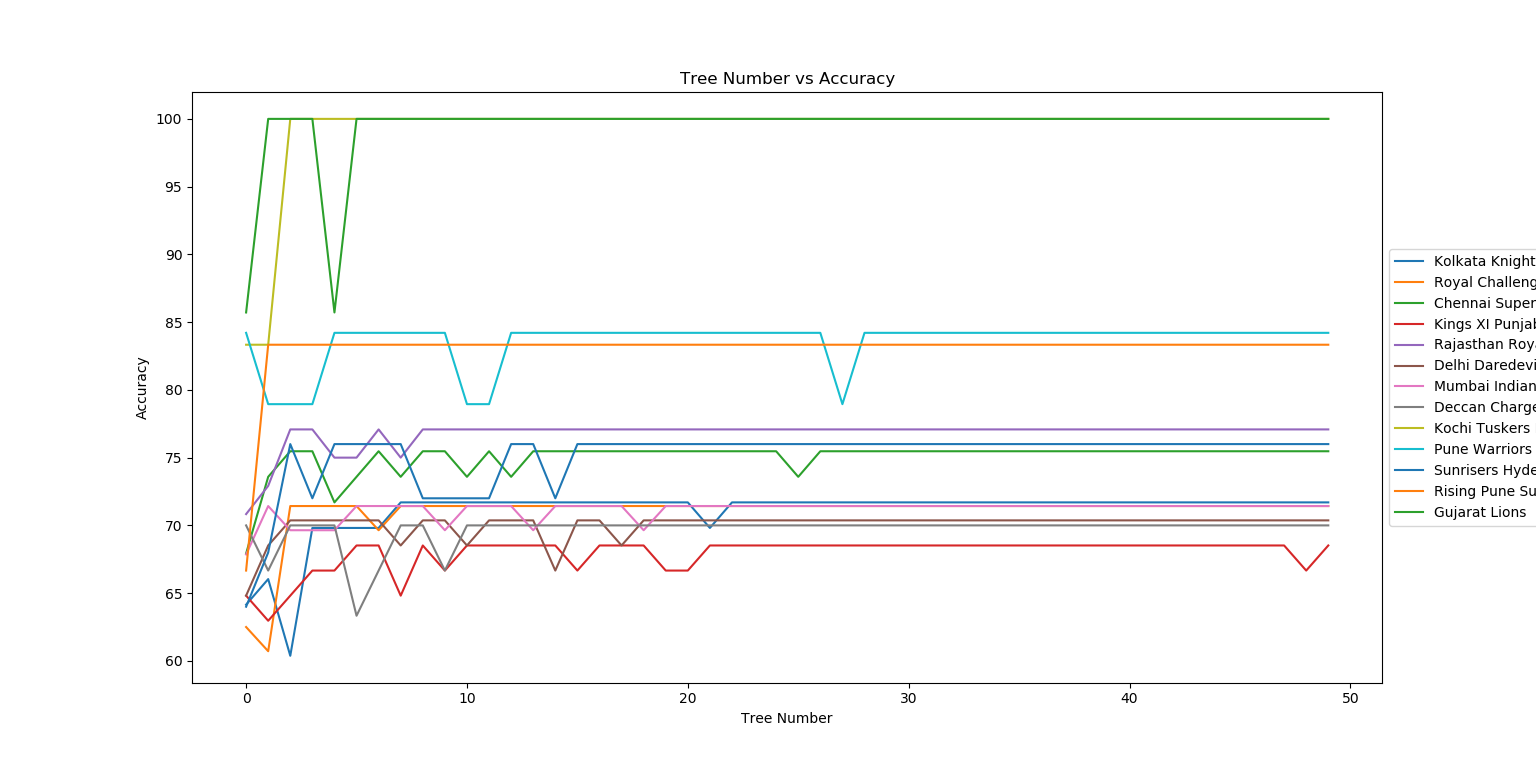
\includegraphics[width=\columnwidth]{images/treenumvsaccuracy.png}
  \caption{Tree number vs Accuracy}\label{f:treenumvsaccuracy}
  
  \centering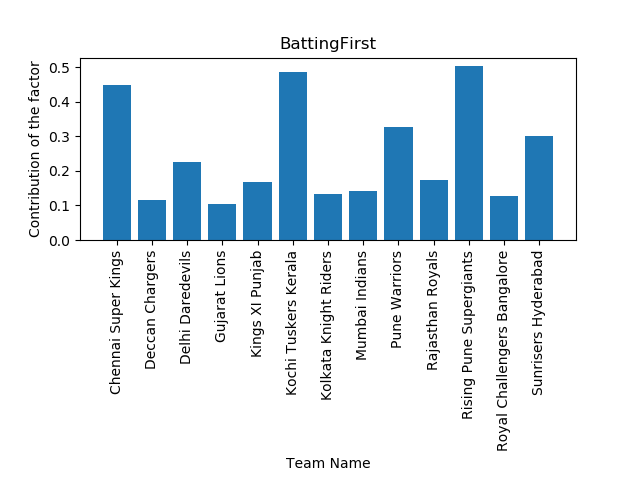
\includegraphics[width=\columnwidth]{images/BattingFirst.png}
  \caption{BattingFirst}\label{f:BattingFirst}
  
  \centering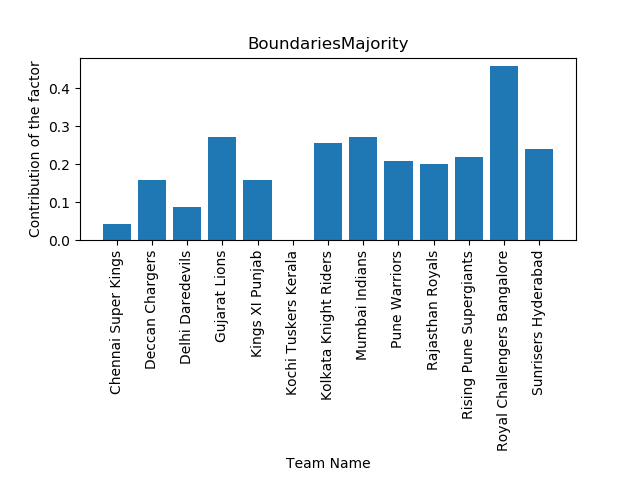
\includegraphics[width=\columnwidth]{images/BoundariesMajority.png}
  \caption{Majority of runs in boundaries}\label{f:BoundariesMajority}
  
  \centering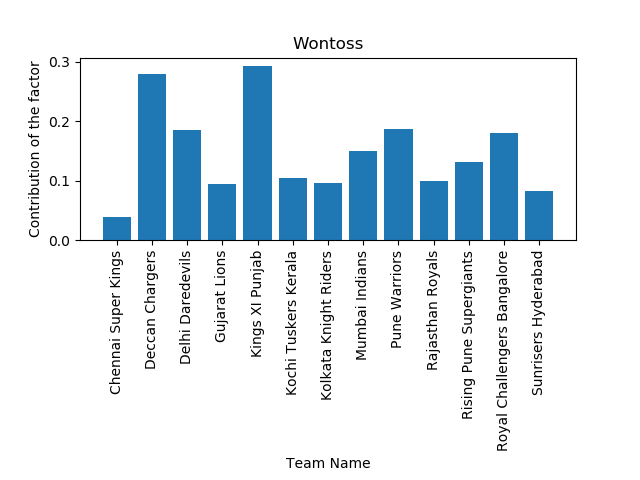
\includegraphics[width=\columnwidth]{images/Wontoss.png}
  \caption{Toss}\label{f:Wontoss}
  
  \centering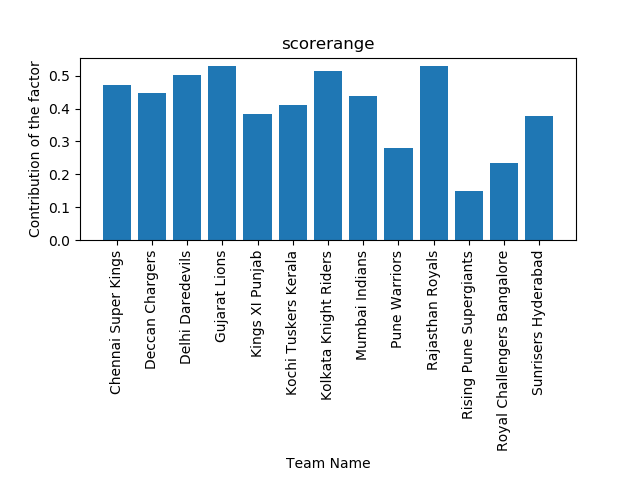
\includegraphics[width=\columnwidth]{images/scorerange.png}
  \caption{Range of Scores}\label{f:scorerange}
\end{figure}


\end{document}
